
\section*{Схема алгоритма} 

\begin{figure}[h!]
	\begin{center}
		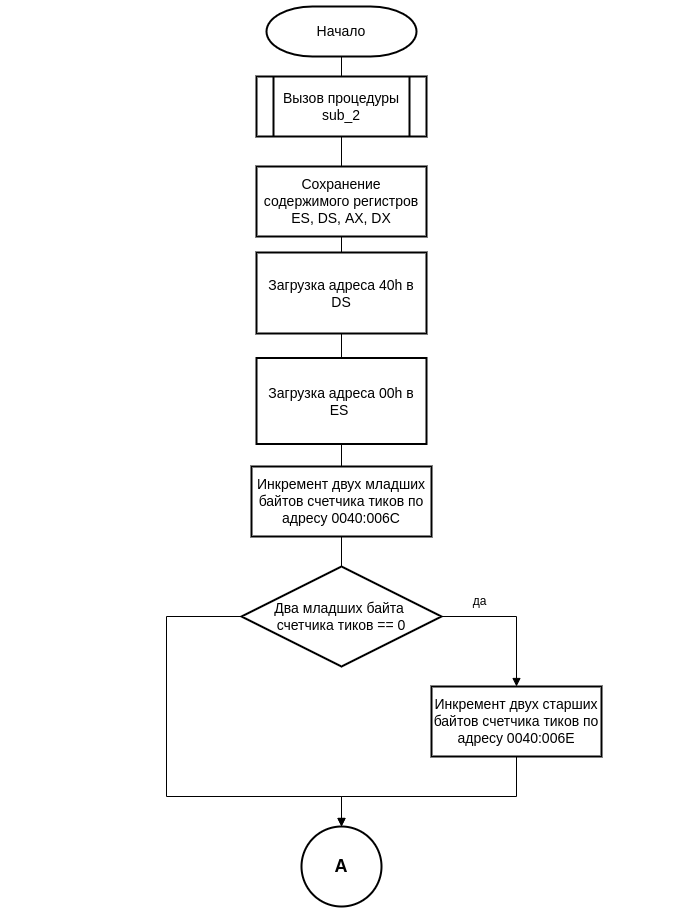
\includegraphics[scale=0.6]{img/int8h_1}
	\end{center}
	\captionsetup{justification=centering}
	\caption{Схема обработчика прерываний INT 8h}
	\label{img:s1}
\end{figure}

\begin{figure}[h!]
	\begin{center}
		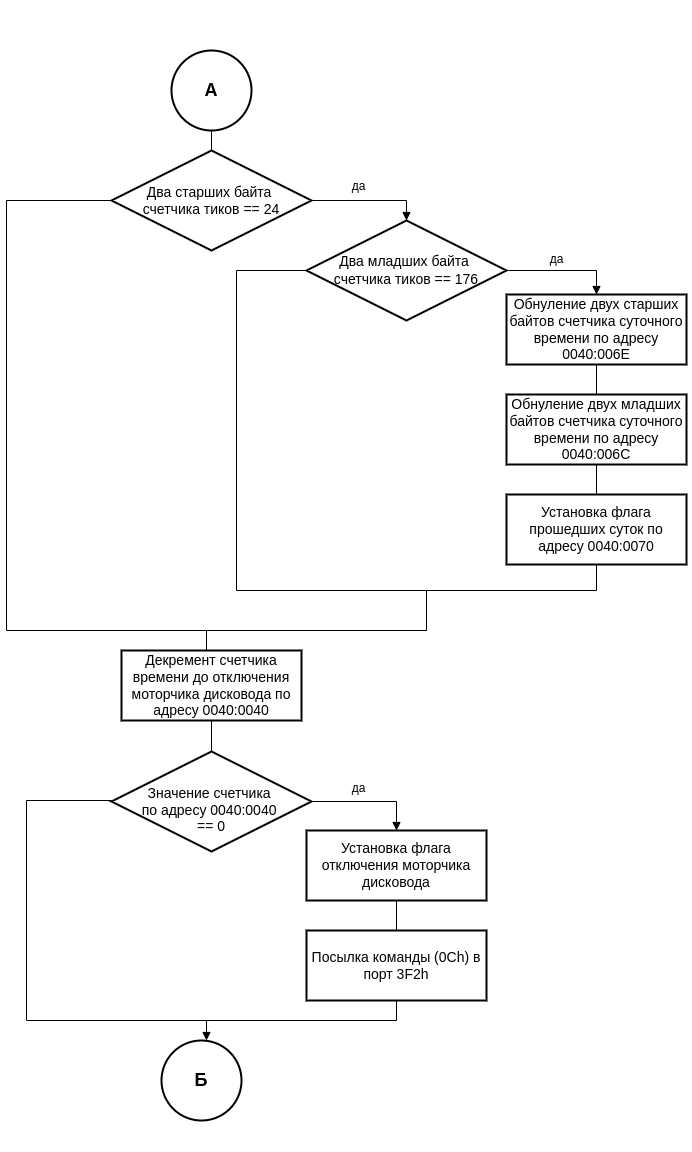
\includegraphics[scale=0.6]{img/int8h_2}
	\end{center}
	\captionsetup{justification=centering}
	\caption{Схема обработчика прерываний INT 8h}
	\label{img:s1}
\end{figure}

\begin{figure}[h!]
	\begin{center}
		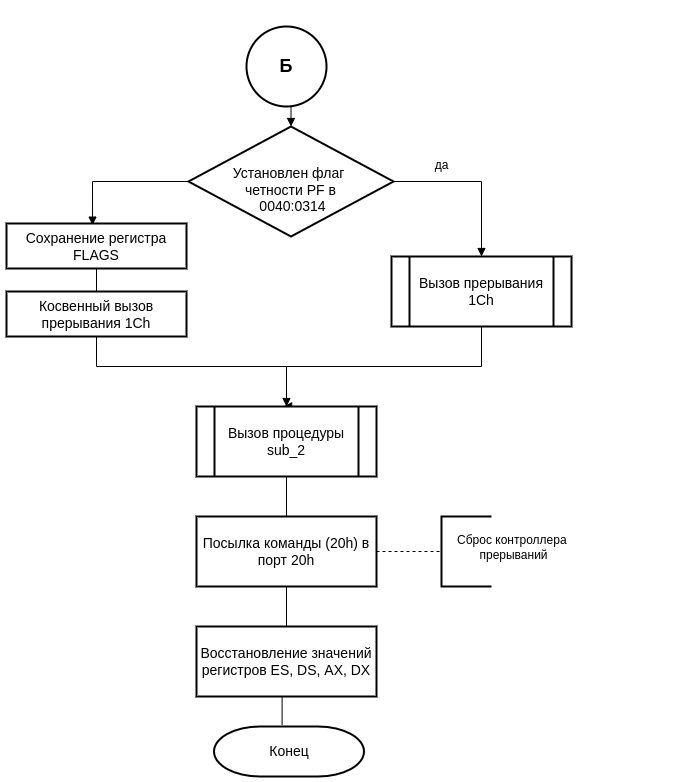
\includegraphics[scale=0.7]{img/int8h_3}
	\end{center}
	\captionsetup{justification=centering}
	\caption{Схема обработчика прерываний INT 8h}
	\label{img:s1}
\end{figure}



\begin{figure}
	\begin{center}
		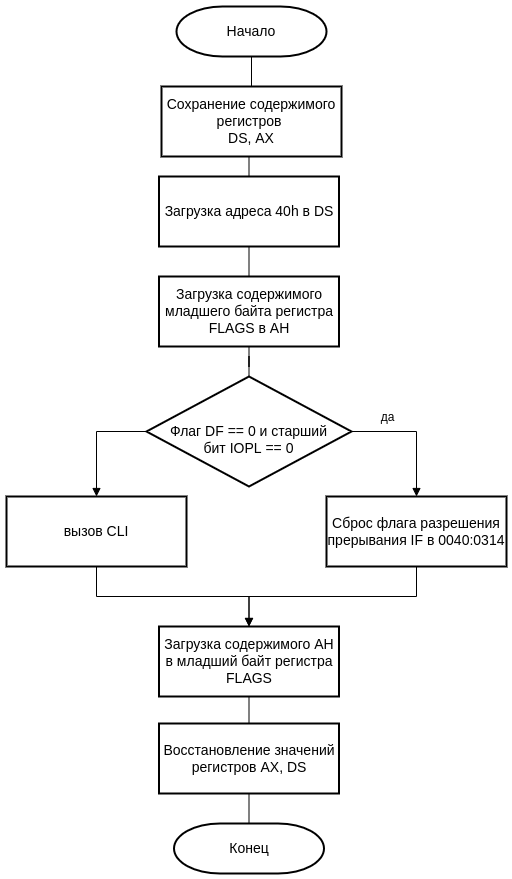
\includegraphics[scale=0.7]{img/sub_2}
	\end{center}
	\captionsetup{justification=centering}
	\caption{Схема подпрограммы sub\_2}
	\label{img:s1}
\end{figure}